\chapter{O ar, uma mistura de gases}\label{ch:g4:air-a-mixture-of-gases}

Num dia de vento, uma pipa puxa a linha, e no lago uma vela se enche e
empurra o barco. Alguma coisa está empurrando os dois, mas não há nada
para ver. Essa coisa é o \omterm{def:g4:air-a-mixture-of-gases:air}{ar}. Não conseguimos vê-lo, mas ele está em
toda a nossa volta, enche cada garrafa vazia e cada cômodo, e nós o
puxamos para dentro a cada respiração. De que o \omterm{def:g4:air-a-mixture-of-gases:air}{ar} é feito?

\begin{recall}
\omterm{def:g2:mixing-and-dissolving:mix}{Misturar} é juntar coisas diferentes; o que obtemos é uma mistura dessas
coisas, e nada se perde quando as \omterm{def:g2:mixing-and-dissolving:mix}{misturamos}
(\cref{ch:g2:mixing-and-dissolving}).
\end{recall}

\begin{omfigure}

\includegraphics[width=0.6\linewidth]{images/book1/ai/g4-kite-day.jpg}

{\small Uma pipa e uma vela: o \omterm{def:g4:air-a-mixture-of-gases:air}{ar} não pode ser visto, mas ele empurra.}
\end{omfigure}

\section{O ar está em toda parte}

\begin{example}[Um copo de boca para baixo]\label{ex:g4:air-a-mixture-of-gases:glass}
Um lenço de papel seco é empurrado até o fundo de um copo vazio. O copo
é virado de boca para baixo e afundado reto numa tigela com água.
Quando ele é tirado de novo, o lenço continua seco. O copo não estava
vazio: estava cheio de \omterm{def:g4:air-a-mixture-of-gases:air}{ar}, e o \omterm{def:g4:air-a-mixture-of-gases:air}{ar} não deixou a água entrar.
\end{example}

\begin{omfigure}
\begin{tikzpicture}[font=\small, scale=1.3]
  \pic[transform shape] at (0,0) {trough};
  % the upturned glass, rim at y = 0.35, base at y = 2.35
  \fill[white] (-0.8,0.5) rectangle (0.8,0.95);
  \pic[transform shape, rotate=180] at (0,2.35) {beaker={0}{white}};
  % the tissue at the top, inside
  \fill[white, draw=black!45, rounded corners=1.5pt] (-0.4,2.33) -- (-0.3,2.05)
    -- (-0.1,2.12) -- (0.05,1.98) -- (0.25,2.1) -- (0.42,2.02) -- (0.45,2.33) -- cycle;
  \draw[<-, omProp, thick] (0.45,2.12) -- (2.4,2.5) node[right, text=black]
    {um lenço seco};
  \draw[<-, omProp, thick] (0.3,1.2) -- (2.4,1.4) node[right, text=black]
    {ar: ele não deixa a água entrar};
  \draw[<-, omProp, thick] (1.4,0.7) -- (2.4,0.55) node[right, text=black]
    {água};
\end{tikzpicture}

{\small O copo é afundado de boca para baixo na água. O \omterm{def:g4:air-a-mixture-of-gases:air}{ar} preso lá
dentro não deixa a água entrar, e o lenço continua seco.}
\end{omfigure}


\begin{remark}[O ar é um gás]\label{rem:g4:air-a-mixture-of-gases:gas}
O \omterm{def:g4:air-a-mixture-of-gases:air}{ar} é um gás: ele não tem forma própria e se espalha para ocupar
qualquer recipiente. Mesmo assim, ele é matéria, e um balão cheio de \omterm{def:g4:air-a-mixture-of-gases:air}{ar}
pesa um pouquinho mais do que o mesmo balão vazio. O que são os gases,
e por que eles se comportam assim, é contado no livro de física.
\end{remark}

\section{O ar é uma mistura}

\begin{definition}[Ar]\label{def:g4:air-a-mixture-of-gases:air}
O \emph{ar}\index{ar} é a mistura de gases que envolve a Terra. Ele não
é um gás só: vários gases estão \omterm{def:g2:mixing-and-dissolving:mix}{misturados} nele, e eles podem ser
separados uns dos outros.
\end{definition}

\begin{proposition}[De que o ar é feito]\label{prop:g4:air-a-mixture-of-gases:composition}
% ledger: air:N2, air:O2, air:Ar, air:trace, air:CO2, air:H2O
Deixando de lado o vapor de água, o \omterm{def:g4:air-a-mixture-of-gases:air}{ar} é feito de:
\begin{itemize}
  \item \textbf{nitrogênio}, cerca de quatro quintos do \omterm{def:g4:air-a-mixture-of-gases:air}{ar};
  \item \textbf{oxigênio}, cerca de um quinto do \omterm{def:g4:air-a-mixture-of-gases:air}{ar};
  \item um pouco de \textbf{argônio}, cerca de 1 parte em 100;
  \item um tantinho de \textbf{dióxido de carbono}, cerca de 4 partes em
        10\,000, e quantidades minúsculas de outros gases.
\end{itemize}
O \omterm{def:g4:air-a-mixture-of-gases:air}{ar} também contém \textbf{vapor de água}, invisível: muito pouco num
dia frio e seco, até cerca de 4 partes em 100 num dia quente e úmido.
\end{proposition}

\begin{example}[Cem garrafas de ar]\label{ex:g4:air-a-mixture-of-gases:hundred}
% ledger: air:N2, air:O2, air:Ar
Imagine 100 garrafas de \omterm{def:g4:air-a-mixture-of-gases:air}{ar} seco, e os gases do \omterm{def:g4:air-a-mixture-of-gases:air}{ar} separados em garrafas
diferentes. Cerca de 78 garrafas teriam nitrogênio, 21 garrafas
oxigênio, e a última garrafa argônio, com o equivalente a umas gotinhas
de dióxido de carbono e de outros gases.
\end{example}

\begin{omfigure}
\begin{tikzpicture}[font=\small, x=0.42cm, y=0.42cm]
  \foreach \k in {0,...,99} {
    \pgfmathtruncatemacro\col{mod(\k,10)}
    \pgfmathtruncatemacro\row{9-int(\k/10)}
    \ifnum\k<78 \def\c{omDef!45}\else\ifnum\k<99 \def\c{red!45}\else\def\c{cyan!60}\fi\fi
    \fill[\c, draw=white, line width=0.8pt] (\col,\row) rectangle ++(1,1);
  }
  \fill[omDef!45] (12,8) rectangle ++(1,1);
  \node[anchor=west] at (13.3,8.5) {nitrogênio: 78 quadrados};
  \fill[red!45] (12,6) rectangle ++(1,1);
  \node[anchor=west] at (13.3,6.5) {oxigênio: 21 quadrados};
  \fill[cyan!60] (12,4) rectangle ++(1,1);
  \node[anchor=west, align=left] at (13.3,4.5) {argônio, dióxido de carbono\\ e o resto: 1 quadrado};
\end{tikzpicture}

{\small Cem quadrados de \omterm{def:g4:air-a-mixture-of-gases:air}{ar} seco. O quadrado lá embaixo, à direita,
contém o argônio e o dióxido de carbono, pequeno demais para ser
desenhado sozinho.}
\end{omfigure}

\begin{remark}[Nomes de gases]\label{rem:g4:air-a-mixture-of-gases:names}
Nitrogênio, oxigênio, argônio e dióxido de carbono são nomes de gases.
Todos eles são incolores e não têm cheiro. Um capítulo mais adiante
mostra de que cada um deles é feito, até os pedacinhos minúsculos que
formam toda a matéria.
\end{remark}

\section{O ar que inspiramos e expiramos}

\begin{proposition}[O ar expirado]\label{prop:g4:air-a-mixture-of-gases:breath}
% ledger: breath:O2, breath:CO2, breath:N2, air:O2, air:CO2
O \omterm{def:g4:air-a-mixture-of-gases:air}{ar} que soltamos não é o \omterm{def:g4:air-a-mixture-of-gases:air}{ar} que puxamos. Nosso corpo fica com uma
parte do oxigênio e solta dióxido de carbono e vapor de água:
\begin{itemize}
  \item cerca de 21 partes em 100 do \omterm{def:g4:air-a-mixture-of-gases:air}{ar} inspirado são oxigênio, mas só
        cerca de 16 partes em 100 do \omterm{def:g4:air-a-mixture-of-gases:air}{ar} expirado;
  \item o dióxido de carbono passa de cerca de 4 partes em 10\,000 para
        cerca de 4 partes em 100: umas cem vezes mais;
  \item o nitrogênio é expirado do mesmo jeito que foi inspirado.
\end{itemize}
\end{proposition}

\begin{omfigure}
\begin{tikzpicture}
\begin{axis}[ybar, width=0.8\linewidth, height=5.2cm, bar width=12pt,
    ymin=0, ymax=90, ylabel={partes em 100},
    symbolic x coords={nitrogen, oxygen, carbon dioxide}, xtick=data,
    xticklabels={nitrogênio, oxigênio, dióxido de carbono},
    tick label style={font=\small}, label style={font=\small},
    xticklabel style={text height=1.6ex, text depth=0.4ex},
    legend style={font=\small, at={(0.98,0.95)}, anchor=north east},
    nodes near coords, nodes near coords style={font=\footnotesize},
    enlarge x limits=0.25, axis lines*=left, ymajorgrids,
    grid style={gray!20}]
% ledger: air:N2, air:O2, air:CO2, breath:N2, breath:O2, breath:CO2 (rounded)
\addplot[fill=omDef!45, draw=omDef] coordinates
  {(nitrogen,78) (oxygen,21) (carbon dioxide,0)};
\addplot[fill=omProp!55, draw=omProp] coordinates
  {(nitrogen,78) (oxygen,16) (carbon dioxide,4)};
\legend{inspirado, expirado}
\end{axis}
\end{tikzpicture}

{\small O \omterm{def:g4:air-a-mixture-of-gases:air}{ar} inspirado e o \omterm{def:g4:air-a-mixture-of-gases:air}{ar} expirado, em partes em 100 (sem o vapor de
água, números arredondados). O dióxido de carbono do \omterm{def:g4:air-a-mixture-of-gases:air}{ar} inspirado,
4 partes em 10\,000, é pequeno demais para aparecer como barra.}
\end{omfigure}

\begin{example}[Uma sala cheia de gente]\label{ex:g4:air-a-mixture-of-gases:room}
Numa sala de aula pequena com as janelas fechadas, trinta pessoas soltam
dióxido de carbono a manhã inteira. Pouco a pouco, o \omterm{def:g4:air-a-mixture-of-gases:air}{ar} da sala passa a
ter menos oxigênio e mais dióxido de carbono, e as pessoas se sentem
cansadas. Abrir as janelas traz \omterm{def:g4:air-a-mixture-of-gases:air}{ar} fresco de volta.
\end{example}

\begin{omfigure}
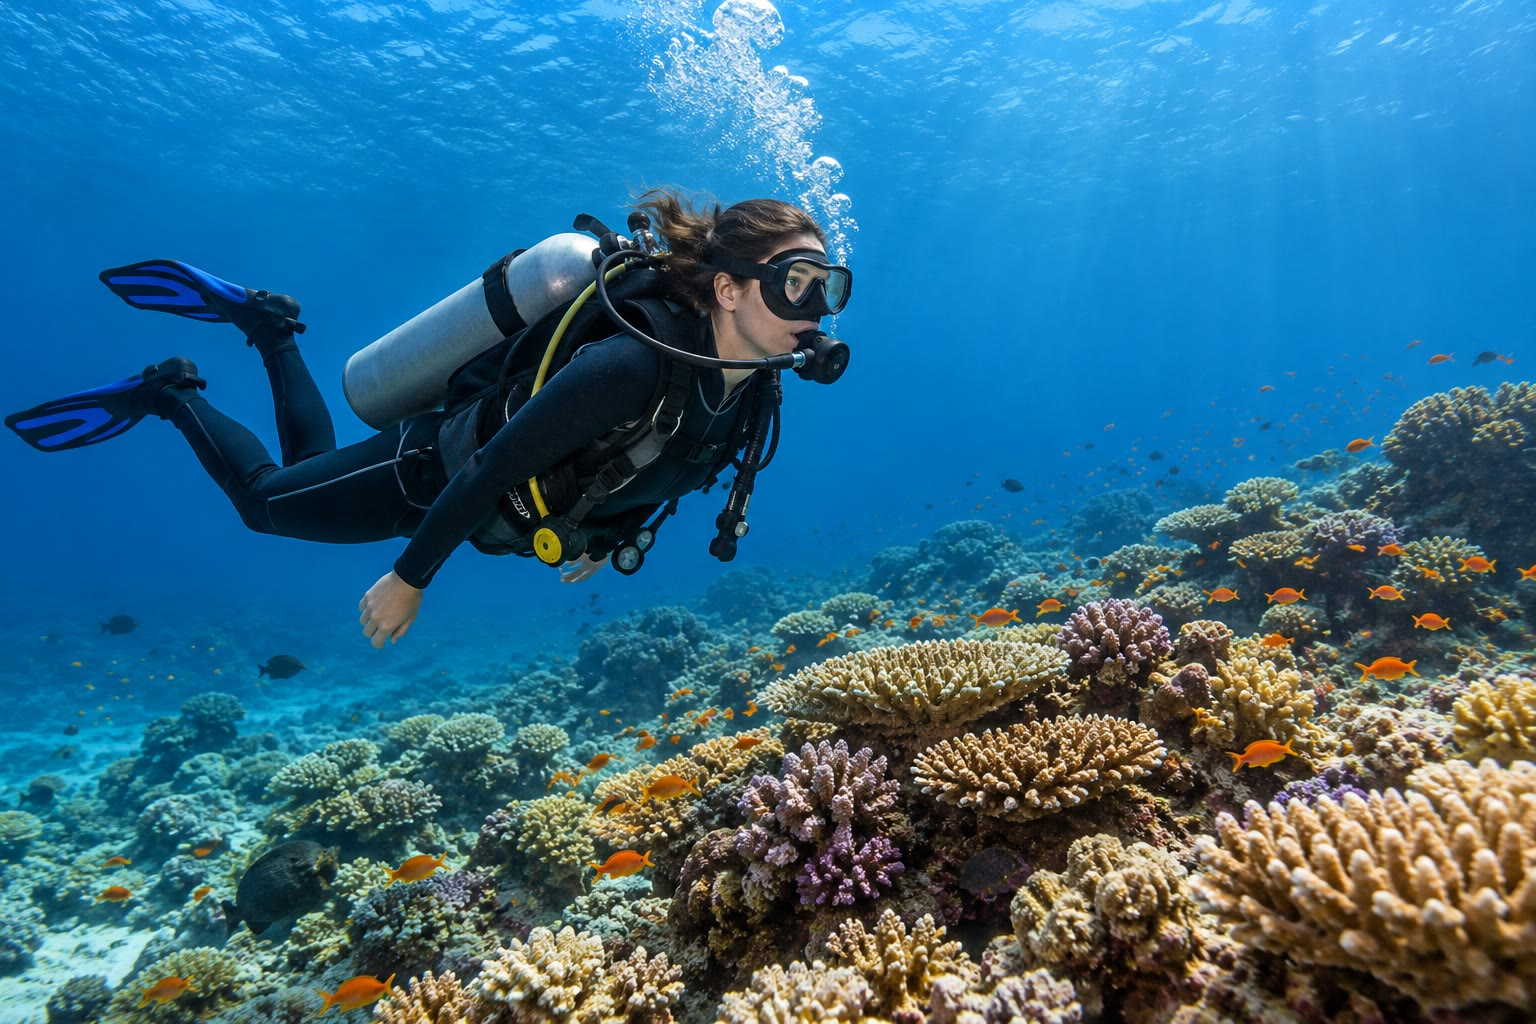
\includegraphics[width=0.55\linewidth]{images/book1/ai/g4-scuba-diver.jpg}

{\small Um mergulhador respira o \omterm{def:g4:air-a-mixture-of-gases:air}{ar} do cilindro que leva nas costas; as
bolhas são o \omterm{def:g4:air-a-mixture-of-gases:air}{ar} expirado.}
\end{omfigure}

\begin{remark}[Por que os mergulhadores respiram ar]\label{rem:g4:air-a-mixture-of-gases:diver}
O cilindro de um mergulhador é enchido com \omterm{def:g4:air-a-mixture-of-gases:air}{ar} apertado num espaço
pequeno, e não com oxigênio puro: respirar oxigênio puro no fundo da
água é perigoso. O nitrogênio do \omterm{def:g4:air-a-mixture-of-gases:air}{ar} está lá para diluir o oxigênio.
\end{remark}

\section{O oxigênio da vida e do fogo}

\begin{proposition}[O oxigênio é consumido pelos seres vivos e pelas chamas]\label{prop:g4:air-a-mixture-of-gases:oxygen}
De todos os gases do \omterm{def:g4:air-a-mixture-of-gases:air}{ar}, o oxigênio é aquele de que os seres vivos e as
chamas precisam. Os animais e as pessoas o puxam quando respiram; uma
chama o tira do \omterm{def:g4:air-a-mixture-of-gases:air}{ar} em volta dela. As plantas verdes, de dia, devolvem
oxigênio ao \omterm{def:g4:air-a-mixture-of-gases:air}{ar}.
\end{proposition}

\begin{inthelab}[Uma vela debaixo de um pote]
O professor acende uma vela em cima de um azulejo e abaixa devagar um
grande pote de vidro sobre ela. A chama diminui, treme e se apaga depois
de alguns segundos: em volta da chama, o \omterm{def:g4:air-a-mixture-of-gases:air}{ar} tem pouco oxigênio demais
para mantê-la acesa. Debaixo de um pote duas vezes maior, a vela queima
cerca de duas vezes mais tempo, porque há cerca de duas vezes mais \omterm{def:g4:air-a-mixture-of-gases:air}{ar},
e portanto duas vezes mais oxigênio, para consumir.
\end{inthelab}

\begin{omfigure}
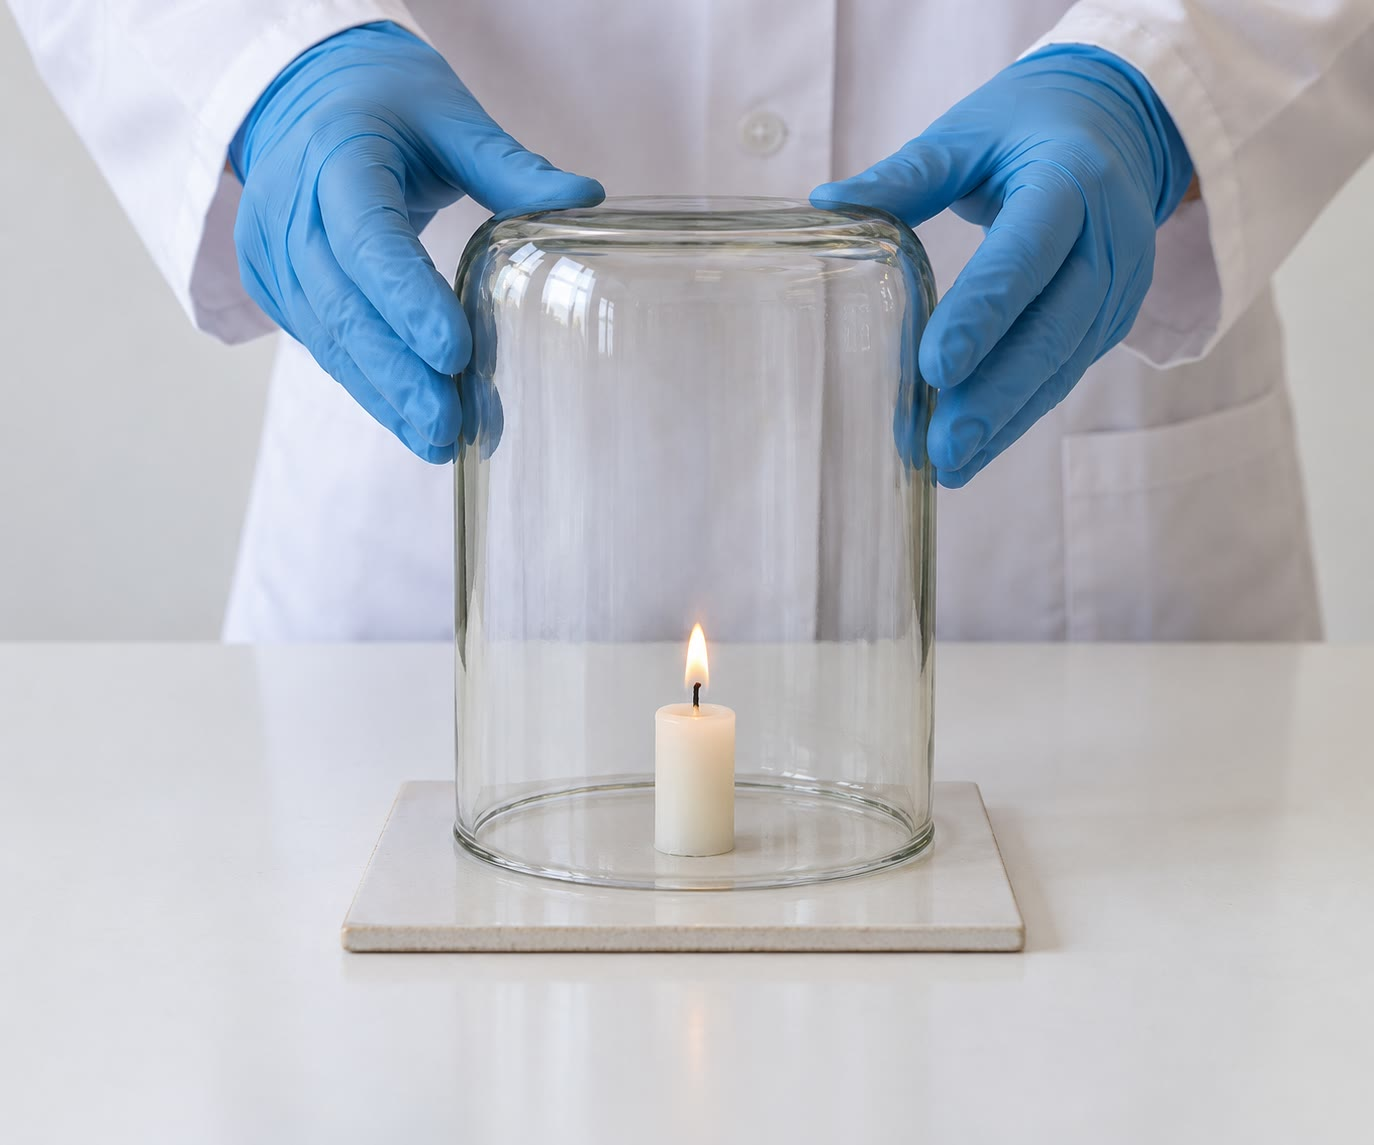
\includegraphics[width=0.5\linewidth]{images/book1/ai/g4-candle-jar-lab.jpg}

{\small Uma vela debaixo de um pote de vidro se apaga quando sobra pouco
oxigênio demais em volta da chama.}
\end{omfigure}

\begin{remark}[O nitrogênio não queima]\label{rem:g4:air-a-mixture-of-gases:nitrogen}
O nitrogênio é a maior parte do \omterm{def:g4:air-a-mixture-of-gases:air}{ar}, mas ele não mantém uma chama acesa e
não é usado pelo nosso corpo. Se o \omterm{def:g4:air-a-mixture-of-gases:air}{ar} fosse só nitrogênio, não
poderíamos respirar e nada poderia queimar.
\end{remark}

\section{Exercícios}

\begin{exercise}[$\star$]\label{exo:g4:air-a-mixture-of-gases:1}
O \omterm{def:g4:air-a-mixture-of-gases:air}{ar} é um gás só ou uma mistura? Diga os dois principais gases do \omterm{def:g4:air-a-mixture-of-gases:air}{ar}.
\end{exercise}

\begin{exercise}[$\star$]\label{exo:g4:air-a-mixture-of-gases:2}
Mais ou menos que fração do \omterm{def:g4:air-a-mixture-of-gases:air}{ar} é nitrogênio? Mais ou menos que fração
é oxigênio?
\end{exercise}

\begin{exercise}[$\star$]\label{exo:g4:air-a-mixture-of-gases:3}
Em 100 litros de \omterm{def:g4:air-a-mixture-of-gases:air}{ar} seco, mais ou menos quantos litros são nitrogênio?
Mais ou menos quantos litros são oxigênio?
\end{exercise}

\begin{exercise}[$\star$]\label{exo:g4:air-a-mixture-of-gases:4}
Uma garrafa vazia é afundada de boca para baixo numa bacia com água.
Por que a água não enche a garrafa?
\end{exercise}

\begin{exercise}[$\star$]\label{exo:g4:air-a-mixture-of-gases:5}
Olhe o gráfico de barras. De que gás há menos no \omterm{def:g4:air-a-mixture-of-gases:air}{ar} expirado? De que gás
há mais?
\end{exercise}

\begin{exercise}[$\star$]\label{exo:g4:air-a-mixture-of-gases:6}
De que gás do \omterm{def:g4:air-a-mixture-of-gases:air}{ar} uma chama precisa? De que gás do \omterm{def:g4:air-a-mixture-of-gases:air}{ar} nós precisamos
quando respiramos?
\end{exercise}

\begin{exercise}[$\star$]\label{exo:g4:air-a-mixture-of-gases:7}
Olhe a figura dos 100 quadrados. Quantos quadrados são nitrogênio?
Quantos não são nitrogênio?
\end{exercise}

\begin{exercise}[$\star$]\label{exo:g4:air-a-mixture-of-gases:8}
Por que uma vela debaixo de um pote se apaga depois de um tempo?
\end{exercise}

\begin{exercise}[$\star$]\label{exo:g4:air-a-mixture-of-gases:9}
Em 500 litros de \omterm{def:g4:air-a-mixture-of-gases:air}{ar}, mais ou menos quantos litros são oxigênio? (Um
quinto do \omterm{def:g4:air-a-mixture-of-gases:air}{ar} é oxigênio.)
\end{exercise}

\begin{exercise}[$\star\star$]\label{exo:g4:air-a-mixture-of-gases:10}
Por que é uma boa ideia abrir as janelas de uma sala de aula entre uma
aula e outra?
\end{exercise}

\begin{exercise}[$\star\star$]\label{exo:g4:air-a-mixture-of-gases:11}
Uma vela queima durante 10 segundos debaixo de um pote pequeno. Mais ou
menos quanto tempo ela queimaria debaixo de um pote com três vezes mais
\omterm{def:g4:air-a-mixture-of-gases:air}{ar}?
\end{exercise}
